\documentclass[12pt]{article}

\usepackage[utf8]{inputenc}
\usepackage[T1]{fontenc}
\usepackage[letterpaper, margin=1in]{geometry}
\usepackage{setspace}
\usepackage{sectsty}
\usepackage{amsmath,amsfonts,amssymb}
\usepackage{newtxtext,newtxmath}
\usepackage{inter}
\usepackage{multicol}
\usepackage{listings}
\usepackage{xcolor}
\usepackage{caption}
\usepackage{graphicx}

\captionsetup{font=small}

\definecolor{background}{HTML}{F3F3F3}
\definecolor{keyword}{HTML}{007ACC}

\lstdefinestyle{cppstyle}{
	backgroundcolor=\color{background},
	keywordstyle=\color{keyword},
	basicstyle=\ttfamily\footnotesize,
	breakatwhitespace=false,
	breaklines=true,
	keepspaces=true,
	showstringspaces=false,
	showtabs=false,
	tabsize=2,
	captionpos=b
}

\lstset{style=cppstyle}

\usepackage[spanish, es-tabla]{babel}

\usepackage{tikz}
\usepackage{pgfplots, pgfplotstable}
\usepgfplotslibrary{statistics}

\renewcommand{\lstlistingname}{Codigo}
\renewcommand{\lstlistlistingname}{Lista de \lstlistingname s}


\usepackage[backend=bibtex,style=numeric,sorting=none]{biblatex}
\addbibresource{referencias.bib}

\title{Simulador de Cache en C++}
\author{Gerardo Diaz \and Luis Sandoval}
\onehalfspacing
\allsectionsfont{\sffamily\interextrabold }

\begin{document}
\maketitle
%
La caché es una memoria de acceso rápido utilizada en los sistemas informáticos para mejorar el rendimiento del procesador al almacenar temporalmente la información más utilizada. Su uso reduce el tiempo de acceso a la memoria principal y acelera el procesamiento de datos.

En este contexto, se presenta un simulador de caché implementado en C++, con el objetivo de evaluar el rendimiento de diferentes configuraciones y políticas de reemplazo de caché. El simulador se ha diseñado para trabajar con una longitud estándar de 32 \textit{bits} por dirección y bloques de 4 palabras, y permite configurar el tamaño de la memoria caché en \textit{kilobytes}, la cantidad de vías de asociatividad, y la generación de direcciones en distribuciones como uniforme, normal y zipf. Además, se evalúa el efecto de estrategias de optimización como el \textit{prefetching}, en el desempeño del simulador.
%
\section*{Entorno de Ejecución}
\vspace{-5pt}
El simulador de caché en C++ funciona en sistemas operativos Windows y Linux. Para su correcta ejecución, se requiere que el sistema tenga instalado un compilador de C++ y las herramientas de construcción correspondientes, como make o cmake.

Para ejecutar el simulador, se pueden seguir dos opciones. La primera es ejecutar el programa desde la línea de comandos en la terminal, proporcionando los parámetros de configuración y accediendo a un menú para seguir el uso del programa. La segunda opción es ejecutar el simulador directamente con la configuración definida en el archivo "config.json". Este archivo contiene la configuración de la caché, como el tamaño y el número de vías de asociatividad, la política de reemplazo y el tipo de distribución para la generación de direcciones.

La salida del simulador se muestra en la terminal y se genera un archivo de resultados en formato de texto plano llamado "resultados.out". Además, si se utiliza una distribución de direcciones que genera múltiples ejecuciones de simulación, se genera un archivo CSV llamado "nombre-distribucion.csv", que contiene la cantidad de accesos a la cache y la tasa de aciertos en cada ejecución.
%
\section*{Funcionamiento de la Cache}
\vspace{-5pt}
El programa está compuesto por varias clases que emulan el comportamiento de la caché, tales como \lstinline|CacheRequest|, \lstinline|CacheLine|, \lstinline|BaseCache| y \lstinline|SetAssociativeCache|.
%
\subsection*{CacheRequest}
\vspace{-5pt}
La clase es una utilidad que simula las solicitudes de memoria realizadas por la CPU a la caché. Su constructor recibe una dirección de 32 \textit{bits} en formato binario, así como el tamaño en \textit{bits} del \textit{offset} (desplazamiento) y del \textit{set} (conjunto o línea) correspondientes. A partir de esta información, el constructor transforma la dirección en binario en valores binarios que representan el \textit{offset}, el \textit{set} y el \textit{tag}, los cuales son procesados en una línea de la caché.
\vspace{5pt}
\begin{lstlisting}[language=C++, caption={Declaración de la Clase \lstinline|CacheRequest|}]
class CacheRequest
{
private:
	long binaryAddress;
	long tag;
	long set;
	long offset;
	size_t bitsInTag;
	size_t bitsInSet;
	size_t bitsInOffset;
public:
	CacheRequest(long binaryAddress, long offsetBits, long setBits);
	long getTag();
	long getSet();
	long getOffset();
	long getBinaryAddress();
	long getBitsInTag();
	long getBitsInSet();
	long getBitsInOffset();
	void printRequest();
	~CacheRequest();
};
\end{lstlisting}
\newpage
%
\subsection*{CacheLine}
\vspace{-5pt}
La clase modela los bloques de memoria almacenados en una memoria caché,también conocidos como líneas de caché o bloques del conjunto de caché. Esta clase se encarga de almacenar el bloque solicitado por el procesador, una etiqueta para identificar la solicitud del procesador, un bit de validez para comprobar si el dato almacenado actualmente es válido, un contador de tiempo que indica el momento en que se accedió al bloque (útil para la política LRU) y un contador de acceso que indica el número de veces que se ha accedido al bloque (útil para la política LFU).
\vspace{5pt}
\begin{lstlisting}[language=C++, caption={Declaración de la Clase \lstinline|CacheLine|}]
class CacheLine
{
private:
	long tag;
	bool valid;
	long block;
	size_t accessTime;
	size_t accessCounter;
public:
	CacheLine();
	CacheLine(bool valid);
	CacheLine(long tag, bool valid, long block);
	CacheLine(CacheLine &cacheLine);
	long getTag();
	bool getValid();
	long getBlock();
	long getAccessTime();
	long getAccessCounter();
	void setTag(long tag);
	void setValid(bool valid);
	void setBlock(long block);
	void setAccessTime(size_t accessTime);
	void setAccessCounter(size_t accessCounter);
	~CacheLine();
};
\end{lstlisting}
%
\subsection*{PrefetchBuffer}
\vspace{-5pt}
La clase simula un \textit{buffer} de \textit{prefetching} de adyacencias que tiene como tarea almacenar el bloque siguiente y anterior. Cuando se intenta acceder a una dirección, se busca primero en el \textit{buffer} antes de pasar a la caché directamente. Si la dirección se encuentra en el \textit{buffer}, se considera un acierto. Si no se encuentra, no se considera un fallo, sino que se busca en la caché antes de dar un resultado.

El \textit{buffer} de \textit{prefetching} solo almacena la dirección accedida anteriormente, por lo tanto, las direcciones almacenadas se actualizarán cada vez que se acceda a una nueva dirección. La fórmula utilizada para determinar el bloque siguiente y anterior es:

\begin{align*}
	\textit{bloqueSiguiente} &= D + (W * B * 8)\\
	\textit{bloqueAnterior} &= D - (W * B * 8)
\end{align*}

Para aplicar esta fórmula, deben cumplirse las siguientes condiciones:

\begin{itemize}
	\item La variable $W$ (tamaño de la palabra en \textit{bytes}) debe ser mayor o igual a 1.
	
	\item La variable $B$ (tamaño del bloque en palabras) debe ser mayor o igual a 1.
	
	\item La variable $D$ (dirección del bloque actual) debe ser mayor o igual a 0 y menor o igual a $2^{32}-1$.
	
	\item La variable \textit{bloqueSiguiente}, que se define como $D + (W * B * 8)$, debe ser mayor o igual a $D$ y menor o igual a $2^{32}-1$.
	
	\item La variable \textit{bloqueAnterior}, que se define como $D - (W * B * 8)$, debe ser mayor o igual a 0 y menor o igual a $D$.
\end{itemize}

Es importante tener en cuenta que no siempre existirá un bloque siguiente o anterior, como en el caso que $(D = 2^{32} - 1) \lor (D = 0)$
\vspace{5pt}
\begin{lstlisting}[language=C++, caption={Declaración de la Clase \lstinline|PrefetchBuffer|}]
class PrefetchBuffer
{
private:
	vector<CacheLine> buffer;
	size_t access_time;
	size_t miss_counter;
public:
	PrefetchBuffer();
	long getBufferSize();
	CacheLine getLine(long index);
	bool checkBuffer(long tag);
	void clearBuffer();
	void storeAdjacentBlocks(CacheRequest *request);
	size_t getAccessTime();
	size_t getMissCounter();
	void incrementAccessTime();
	void incrementMissCounter();
};
\end{lstlisting}
%
\subsection*{SetAssociativeCache}
\vspace{-5pt}
Esta clase representa una cache asociativa por conjuntos que contiene métodos para guardar bloques con diferentes políticas de reemplazo en una cache de $N$ bloques divididos en $M$ conjuntos. Además de ello, posee un \textit{buffer} de \textit{prefetching} de adyacencias.
\vspace{5pt}
\begin{lstlisting}[language=C++, caption={Declaración de la Clase \lstinline|SetAssociativeCache|}]
class SetAssociativeCache {
private:
	long n_ways;
	vector<CacheLine> cache;
	long sets_in_cache;
public:
	SetAssociativeCache(long s_block, long s_cache, long n_ways) : n_ways(n_ways), sets_in_cache(s_cache / n_ways) {}
	void saveBlockInCache(long binaryAddress);
	bool insertBlockLFU(long currentBlock, long tag, long address);
	bool insertBlockLRU(long currentBlock, long tag, long address);
	bool insertBlockRandom(long currentBlock, long tag, long address);
	string getFeatures();
	void printFeatures();
};
\end{lstlisting}
%
\subsection*{BaseCache}
\vspace{-5pt}
Clase base que es heredara para implementaciones específicas de una cache. Se ha creado para contener métodos y propiedades comunes en una cache genérica.
%SetAssociativeCache la implementa-%
\vspace{5pt}
\begin{lstlisting}[language=C++, caption={Declaración de la Clase \lstinline|BaseCache|}]
class BaseCache {
protected:
	long s_block;
	long s_cache;
	long blocks_in_cache; torre movilnet
	long sets_in_cache;
	size_t access_time;
	size_t miss_counter;
	long bitsInOffset;
	long bitsInSet;
	long bitsInTag;
	short replacePolicy;
	PrefetchBuffer *prefetchBuffer;
public:
	BaseCache(long s_block, long s_cache, short replacePolicy = 0);
	virtual void saveBlockInCache(long blockAddress) = 0;
	void calculateBlocksInCache();
	double getRealSize(long bitsInTag);
	double getMissRate();
	double getHitRate();
	size_t getAccessTime();
	size_t getTotalAccessTime();
	long getSBlock();
	long getSCache();
	size_t getMissCounter();
	long getBitsInOffset();
	long getBitsInSet();
	long getBitsInTag();
	long getSetsInCache();
	long getBlocksInCache();
	void setSBlock(long s_block);
	void setSCache(long s_cache);
	void setReplacePolicy(short replacePolicy);
	void setAccessTime(size_t access_time);
	void incrementAccessTime();
	void setBlocksInCache(long blocks_in_cache);
	void setSetsInCache(long sets_in_cache);
	void setBitsInOffset(long bitsInOffset);
	void setBitsInSet(long bitsInSet);
	void setBitsInTag(long bitsInTag);
};
\end{lstlisting}
%
\section*{Operaciones}
\vspace{-5pt}
El funcionamiento de la cache se describe a continuación:

\begin{enumerate}
	\item \textbf{Configuración inicial}: La caché se inicializa con los valores proporcionados por el usuario. Estos valores pueden ser ingresados a través de un archivo de configuración o por la entrada estándar del programa. Los valores que se deben especificar incluyen el número de vías de asociatividad, el tamaño total de la caché en \textit{kilobytes}, la política de reemplazo a utilizar y el tipo de distribución para generar las direcciones de prueba de la caché.
	
	\item \textbf{Cálculo de tamaño}: El programa calcula el tamaño necesario en bits para los campos \textit{tag}, \textit{set} y \textit{offset}, así como el número total de bloques en la caché.
	
	\item \textbf{Inicialización}: Todas las posiciones en la caché se inicializan colocando 0 en el bit de invalidez. Esto asegura que ninguna posición sea considerada en las operaciones que se realizan posteriormente.
	
	\item \textbf{Lectura de bloques}: El programa lee los bloques del archivo o del generador de direcciones, y luego llama a la función \lstinline|saveBlockInCache|. Esta función inserta cada bloque en la caché utilizando el algoritmo de reemplazo seleccionado, y también revisa el buffer de prefetching antes de insertar un bloque en la caché. De esta manera, el programa puede aprovechar el prefetching para mejorar la tasa de aciertos de la caché.
	
	\item \textbf{Resultados}: Al finalizar la ejecución, el programa muestra un resumen de los resultados de todas las operaciones por consola y por salida estándar. Este resumen incluye la tasa de fallos, la tasa de aciertos, el número de operaciones, un resumen de las prestaciones de la caché y un archivo en formato CSV que muestra la evolución de las operaciones en términos de tasa de aciertos por número de accesos. De este modo, el usuario puede analizar los resultados de manera detallada y obtener información sobre el rendimiento de la caché.
\end{enumerate}
%
\section*{Benchmark}
\vspace{-5pt}
Se ha desarrollado un archivo en Python 3 con el objetivo de evaluar el rendimiento de las distintas distribuciones de direcciones en diferentes computadoras. Este archivo proporciona una salida estándar del sistema con los siguientes valores:

\begin{itemize}
	\item \textbf{Tiempo de ejecución}: El tiempo real que toma el programa en ejecutarse, lo que significa que se excluye el tiempo que el sistema operativo y el kernel utilizan.
	
	\item \textbf{Uso de CPU}: El tiempo asignado por el sistema operativo para la ejecución del programa, menos el tiempo que se dedica a otros programas durante la ejecución.
	
	\item  \textbf{Uso de RAM}: Es la cantidad total de memoria RAM que utiliza un programa.
\end{itemize}
%
\section*{Entorno de Laboratorio}
\vspace{-5pt}
Para simular el entorno del laboratorio, se utilizaron herramientas como Docker y se evitó el uso de librerías externas o no estándar. Asi mismo, la imagen de Docker utilizada para ejecutar el programa tiene como base Ubuntu 14.04. Los pasos de construcción son los siguientes:

\begin{enumerate}
	\item Se utiliza Ubuntu 14.04 como sistema operativo base.
	
	\item Para compilar el código en C++, es necesario descargar e instalar el compilador g++. Se puede hacer esto en Ubuntu 14.04 con el siguiente comando en la terminal:
	
	\begin{lstlisting}[language=bash]
	sudo apt-get install g++
	\end{lstlisting}

	\item También se instala la utilidad adicional nano con el siguiente comando:
	
	\begin{lstlisting}[language=bash]
	sudo apt-get install nano
	\end{lstlisting}

	\item El código se compila con el comando:
	
	\begin{lstlisting}[language=bash]
	g++ -std=c++11 main.cpp -o RUN.out
	\end{lstlisting}
	
	\item Se ejecuta el script de \textit{benchmarking} en Python, compatible con la versión 3.4.3 que se utiliza en el laboratorio y viene incluida por defecto en Ubuntu 14.04. El comando para ejecutar el script es el siguiente:
	
	\begin{lstlisting}[language=bash]
	python3 cache_time.py
	\end{lstlisting}
	
	\item El script en Python ejecuta automáticamente el archivo compilado en C++ y muestra por pantalla las características mencionadas en la sección anterior.
\end{enumerate}
\newpage
%
\section*{Generación de Direcciones}
\vspace{-5pt}
Para evaluar el rendimiento de la caché, se generan $N$ direcciones de $2^{32}$ \textit{bits}. Estas direcciones se generan utilizando diferentes distribuciones de probabilidad, como la distribución uniforme, normal y de Zipf, incluyendo modificaciones de las mismas. La aleatoriedad en la generación de direcciones depende de la semilla utilizada en el generador de números aleatorios. En este caso, se utiliza \lstinline|std::random_device| para obtener una semilla aleatoria y luego se emplea un generador de números aleatorios Mersenne Twister (\lstinline|std::mt19937|) para generar las direcciones.
\newline

La distribución uniforme genera números aleatorios en un rango determinado, en este caso, de $0$ a $2^{32}-1$ usando \lstinline|std::uniform_int_distribution|. En consecuencia, cada dirección tiene la misma probabilidad de ser generada.
\newline

la distribución normal genera números aleatorios siguiendo una distribución de campana de Gauss usando \lstinline|std::normal_distribution<> distribution(0, 100)|. Por lo tanto, las direcciones generadas estarán más concentradas cerca de la media de la distribución, y su probabilidad disminuirá a medida que se alejen de la media. 

\begin{figure}[h]
	\centering
	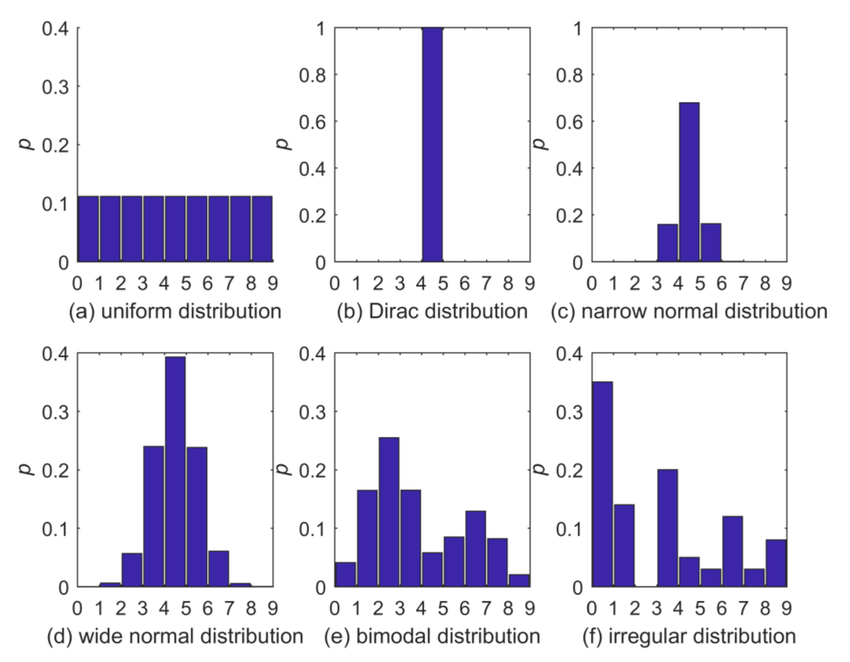
\includegraphics[width=0.8\textwidth]{test-distributions.png}
	\caption{Tipos de Distribuciones \cite{darscheid_maximum-entropy_2018}}
	\label{fig:uni_normal_dist}
\end{figure}

La distribución zipf genera números aleatorios siguiendo la ley de Zipf, que establece que la frecuencia de un elemento es inversamente proporcional a su rango. En este caso, las direcciones generadas estarán más concentradas en un conjunto reducido de valores, mientras que la mayoría de los valores tendrán una frecuencia baja.

\begin{figure}[h]
	\centering
	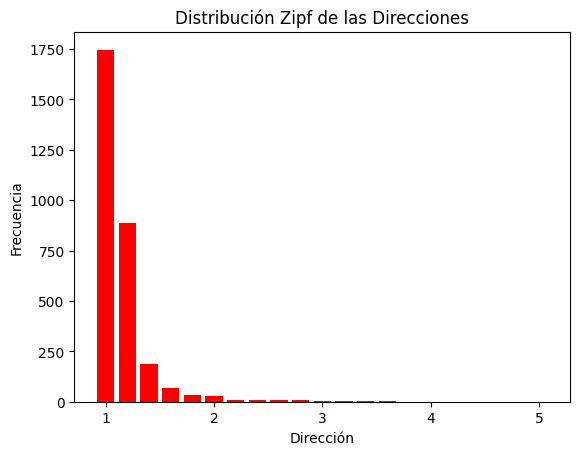
\includegraphics[width=0.57\textwidth]{zipf.png}
	\caption{Distribución Zipf con datos del simulador}
	\label{fig:zipf_dist}
\end{figure}

\begin{figure}[h]
	\centering
	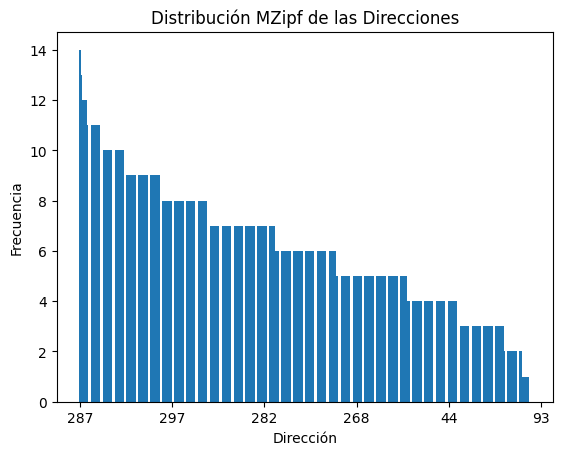
\includegraphics[width=0.57\textwidth]{mzipf.png}
	\caption{Distribución Modified-Zipf con datos del simulador}
	\label{fig:mzipf_dist}
\end{figure}
%
\section*{Discusión de Resultados}
%
\subsection*{Eficacia del Simulador}
\vspace{-5pt}
Para probar el funcionamiento correcto y capacidades del simulador se usó una configuración de 32 \textit{KBytes} de tamaño de caché, 8 vías de asociatividad y LRU como política de reemplazo. Se generaron 3000 direcciones de $2^{32}$ \textit{bits} con 6 implementaciones basadas en las distribuciones explicadas en la sección anterior. Los resultados indican que las distribuciones Zipf y Modified-Zipf, que son las distribuciones más cercanas a la realidad\cite{hefeeda_traffic_2008}, tuvieron las mejores prestaciones.
\newline

\begin{tikzpicture}
	\begin{axis}
		[
		width = {0.8\linewidth},
		title = {Comparación entre Distribuciones},
		xlabel = {Número de Accesos},
		ylabel = {Tasa de Aciertos (\%)},
		xtick distance = {500},
		ytick distance = {10},
		legend pos = {outer north east},
		legend cell align = {left}
		]
		\addplot[only marks, color=red, restrict x to domain=0:3000]
		table[x=AccessCounter,y=HitRate,col sep=comma] {zipf.csv};
		\addlegendentry{Zipf}
		
		\addplot[only marks, color=blue, restrict x to domain=0:3000]
		table[x=AccessCounter,y=HitRate,col sep=comma] {mzipf.csv};
		\addlegendentry{MZipf}
		
		\addplot[only marks, color=teal, restrict x to domain=0:3000]
		table[x=AccessCounter,y=HitRate,col sep=comma] {normal.csv};
		\addlegendentry{Normal}
		
		\addplot[only marks, color=purple, restrict x to domain=0:3000]
		table[x=AccessCounter,y=HitRate,col sep=comma] {augustus.csv};
		\addlegendentry{Augustus}
		
		\addplot[only marks, color=orange, restrict x to domain=0:3000]
		table[x=AccessCounter,y=HitRate,col sep=comma] {uniform2^16.csv};
		\addlegendentry{Uniforme $2^{16}$}
		
		\addplot[only marks, color=yellow, restrict x to domain=0:3000]
		table[x=AccessCounter,y=HitRate,col sep=comma] {uniform2^32.csv};
		\addlegendentry{Uniforme $2^{32}$}
	\end{axis}
\end{tikzpicture}

La distribución Zipf tuvo una tasa de aciertos del 99.83\% y alcanzó el 90\% de aciertos después de 21 accesos. La distribución MZipf consiguió una tasa de aciertos del 98.97\% y alcanzó un 90\% de aciertos después de 311 accesos.
\newline

La distribución uniforme con un rango de 0 a $2^{32}-1$ tuvo el peor resultado de las pruebas, con un 0\% de aciertos. En contraste, la distribución uniforme con un rango de 0 a $2^{16}-1$ obtuvo un mejor desempeño logrando un 21\% y, en pruebas con mayor cantidad de direcciones generadas, se observó que la curva converge en un 48\% de aciertos. Este comportamiento indica que, aunque los valores aleatorios sean generados de forma uniforme, la caché está aprovechando eficazmente la localidad espacial y temporal. En cualquier caso, solo alcanzó acertar la mitad de las veces.
\newline

La distribución Augustus es una distribución uniforme de $2^{32}-1$ con reglas de generación adicionales. En esta distribución, se agrega la posibilidad de repetir valores anteriores y generar valores adyacentes al valor anterior. Esto le permitió hacer uso de las características del \textit{prefetching} y lograr una tasa de aciertos del 81\%.
\newline

La distribución normal alcanzó un 84\% de aciertos en la prueba realizada. No obstante, al incrementar el número de generaciones, se comprobó una convergencia hacia un 96\% debido a la acumulación de valores alrededor de la media, fenómeno que el simulador explotó tanto en el tiempo como en el espacio.
\newline

En conclusión, las distribuciones Zipf y MZipf demostraron un mejor rendimiento en comparación con la distribución uniforme de $2^{32}-1$, que presentó el peor desempeño. Por otro lado, la distribución Augustus aprovechó al máximo las características del \textit{prefetching}, mientras que la distribución normal logró un desempeño promedio gracias a la aplicación de la localidad espacial y temporal en el simulador.
%
\subsection*{Eficiencia del Simulador}
\vspace{-5pt}
Con el fin de evaluar el consumo de recursos informáticos y el tiempo de ejecución, se utilizó la herramienta de \textit{benchmarking} previamente discutida, con la misma configuración empleada en la sección anterior. De igual manera, se generaron 50.000 direcciones de $2^{32}$ bits para realizar esta prueba.

\begin{table}[ht]
	\centering
	\begin{tabular}{|c|c|c|c|}
		\hline
		\multicolumn{4}{|c|}{CPU de 4 núcleos y 3,90 \textit{Ghz} de frecuencia} \\
		\hline
		\textbf{Método de Generación} & \textbf{Tiempo de Ejecución (\textit{s})} & \textbf{Uso de CPU (\%)} & \textbf{Uso de RAM (\textit{MB})} \\
		\hline
		Augustus 			& 16.70  & 5.51 & 26.87 \\
		Uniforme $2^{32}$	& 14.88  & 4.84 & 26.82 \\
		Uniforme $2^{16}$	& 14.05  & 4.84 & 25.84 \\
		Normal 				& 17.01  & 5.64 & 25.97 \\
		Zipf   				& 250.92 & 0.28 & 25.89 \\
		MZipf  				& 16.80  & 5.60 & 25.50 \\
		\hline
		\multicolumn{4}{|c|}{CPU de 2 núcleos y 3,20 \textit{Ghz} de frecuencia} \\
		\hline
		\textbf{Método de Generación} & \textbf{Tiempo de Ejecución (\textit{s})} & \textbf{Uso de CPU (\%)} & \textbf{Uso de RAM (\textit{MB})} \\
		\hline
		Augustus 			& 25.66	 & 4.21 & 26.57 \\
		Uniforme $2^{32}$ 	& 25.07	 & 4.79 & 26.64 \\
		Uniforme $2^{16}$ 	& 25.37	 & 4.73 & 25.41 \\
		Normal 				& 25.68	 & 4.52 & 25.85 \\
		Zipf   				& 450.06 & 0.40 & 26.19 \\
		MZipf  				& 27.03	 & 4.85 & 25.28 \\
		\hline
	\end{tabular}
	\caption{Resultados del \textit{benchmark}}
\end{table}

En general, los resultados obtenidos son coherentes con las características de cada CPU. Sin embargo, se observó una excepción en el caso de la distribución Zipf, la cual requirió un tiempo notablemente mayor. Esta demora se debe a que los cálculos matemáticos necesarios para generar la distribución Zipf son particularmente exigentes en cuanto a recursos computacionales. Para reducir los tiempos de procesamiento, sería necesario aumentar la complejidad de la implementación desarrollada. Por otra parte, la modificación MZipf no presenta este problema, ya que no requiere generar una curva Zipf pura.
%
\vspace{-5pt}
\printbibliography
\end{document}